\documentclass{article}

\usepackage[margin=.55 in]{geometry}
\usepackage{amsmath,amsfonts,textcomp,amssymb,amscd,amsthm,mathrsfs,mathtools}
\usepackage{graphicx,tikz}
\usetikzlibrary{matrix,calc,arrows.meta,angles,quotes,positioning,shapes,fit,backgrounds}
\usepackage{hhline,xcolor}
\usepackage{pgfplots}
\usepackage[mathscr]{euscript}
\pgfplotsset{compat=1.11}

\setlength{\parindent}{0pt}
\setlength{\parskip}{1em}

\DeclareSymbolFont{rsfs}{U}{rsfs}{m}{n}
\DeclareSymbolFontAlphabet{\mathscrsfs}{rsfs}

\makeatletter

\newcommand*\curveplus{%
  \mathbin{\rotatebox[origin=c]{90}{$\m@th\curvearrowleft$}+}}

\newcommand*\rightplus{%
  \mathpalette\@rightplus\relax}
\newcommand*\@rightplus[1]{%
  \mathbin{\vcenter{\hbox{$\m@th\overset{#1+}{\to}$}}}}

\newcommand*\upplus{%
  \mathbin{+\mathord\uparrow}}


\title{Navier-Stokes Equation}
\author{Md. Mesbahose Salekeen}
\date{}

\begin{document}
\maketitle
\large

\section*{Stress}

According to Cauchy hypothesis, the surface (or interface) reaction force acting between
two adjacent portions of a fluid can be characterized by its surface vector density called the
stress.

\begin{figure}[h!]
\centering
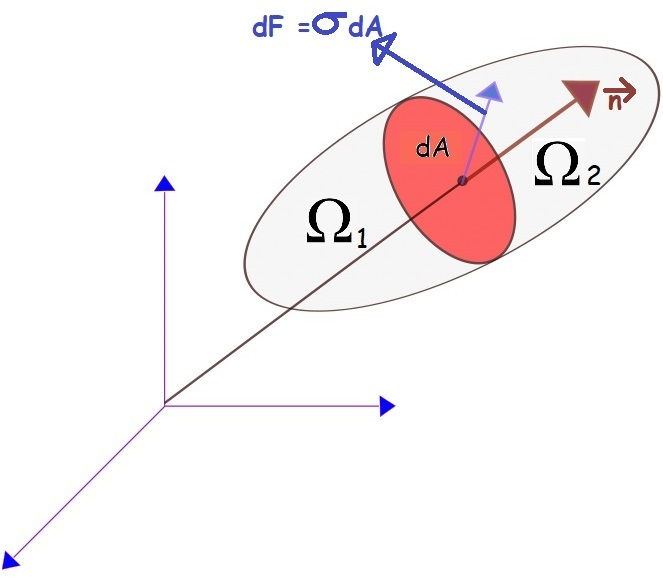
\includegraphics[scale=.4]{Stress.jpg}
\caption{Concept of Stress}
\label{fig:Stress}
\end{figure}

Thus, for an infinitesimal piece dA of the interface $\partial \Omega_{1} \cup \partial \Omega_{2}$, we have

$$dF = \sigma dA \text{ and } F_{\sigma_{2}\to\sigma_{1}} = \int_{\partial \sigma_{1}\cup \partial \sigma_{2}}\sigma dA$$

The stress vector $\sigma$ is not a vector field: it depends not only on the point $x$ but also on the orientation of the surface element $dA$ or – equivalently – on the vector $n$ normal (perpendicular) to $dA$ at the point $x$.

\section*{Viscocity \& Viscous Stress}

Where do stresses come from? For a solid, stresses develop when the material is elastically deformed or strained; for a fluid, shear stresses arise due to viscous flow (we
will discuss a fluid's normal stresses shortly). Hence we say solids are elastic, and
fluids are viscous (and it's interesting to note that many biological tissues are viscoelastic, meaning they combine features of a solid and a fluid). For a fluid at rest,
there will be no shear stresses. We will see that each fluid can be categorized by examining the relation between the applied shear stresses and the flow (specifically the
rate of deformation) of the fluid.

Viscosity is the quantity that describes a fluid's resistance to flow. Fluids resist the relative motion of immersed objects through them as well as to the motion of layers with differing velocities within them.

\begin{figure}[h]
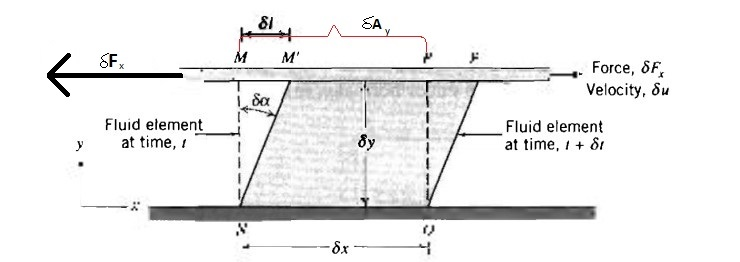
\includegraphics[width=\linewidth]{schematic for viscousity.jpg}
\caption{Deformation of a Fluid Element}
\label{fig:schem_vis}
\end{figure}

Let's consider the fluid element between two parallel infinite plates. The upper plate moves at a constant velocity $\delta u$ under the influence of constant applied force $\delta F_{x}$ due to viscoucity. The shear stress $\tau_{yx}$ developed on the fluid element is given by

$$\tau_{yx} = \lim_{\delta A_{y} \to 0} \frac{\delta F_{x}}{\delta A_{y}} = \frac{\text{d}F_{x}}{\text{d}A_{y}}$$

where $\delta A_{y}$ is the area of contact of a fluid element with the plate, $\delta F_{x}$ is the force exerted by the plate on that element. During time interval 8t, the fluid element is deformed from position MNOP to position M'NOP'. The rate of deformation of the
fluid is given by

$$\text{deformation rate =} \lim_{\delta t \to 0} \frac{\delta \alpha}{\delta t} = \frac{\text{d}\alpha}{\text{d}t}$$

We want to express daldt in terms of readily measurable quantities. This can be done easily. The distance, 81, between the points M and M' is given by

$$\delta l = \delta u\delta t$$

Also from Figure \ref{fig:schem_vis} 

$$\tan(\delta \alpha) = \frac{\delta l}{\delta y} = \delta \alpha, \quad \text{ when } \delta \alpha \text{ is very small}$$ 

$$\therefore \delta l = \delta\alpha \delta y$$

$$\delta u \delta t = \delta \alpha \delta y \Rightarrow \frac{\delta\alpha}{\delta t} = \frac{\delta u}{\delta y}$$

Taking the limits of both sides of the equality, we obtain

$$\frac{\text{d}\alpha}{\text{d}t} = \frac{\text{d}u}{\text{d}y}$$

Thus, the fluid element of \ref{fig:schem_vis} when subjected to shear stress, $\tau_{yx}$, experiences a rate of deformation {shear rate) given by $\frac{\text{d}u}{\text{d}y}$. We have established that any fluid
that experiences a shear stress will flow (it will have a shear rate). What is the relation between shear stress and shear rate? Fluids in which shear stress is directly
proportional to rate of deformation are Newtonian fluids. The term non-Newtonian
is used to classify all fluids in which shear stress is not directly proportional to
shear rate.

For non-newtonian fluid $\tau_{yx} \propto \frac{\text{d}u}{\text{d}y}$

So, viscous stress 

\begin{equation}
\tau_{yx} = \mu\frac{\text{d}u}{\text{d}y} \label{e1}
\end{equation}

\section*{Surface Stress}

The density $\rho(\overrightarrow{x},t)$ is a scalar field in the sense that it has a scalar value at every point, while the velocity $v(\overrightarrow{x},t)$ is a vector field, since it has a direction as well as a magnitude at every point.

\begin{figure}[h]
\centering
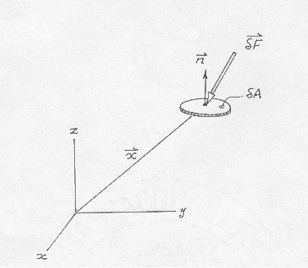
\includegraphics[scale=.8]{surface element in continuum.jpg}
\caption{A surface element at a point in a continuum}
\label{fig:sur_el_in_contnm}
\end{figure}


The surface stress is a more complicated type of quantity. The reason for this is
that one cannot talk of a stress at a point without first defining the particular surface
through that point on which the stress acts. A small fluid surface element centered at the
point $\overrightarrow{r}$ is defined by its area $\delta A$ and its unit outward normal vector $\overrightarrow{n}$ (the prefix $\delta$ indicates an infinitesimally small quantity). The stress exerted on the surface element by the adjacent fluid on the side toward which $\overrightarrow{n}$ points is defined as

\begin{equation}
\bar{\sigma} = \lim_{\delta A \to 0} \frac{\delta \overrightarrow{F}}{\delta A} \label{e2}
\end{equation}

where $\delta \overrightarrow{F}$ is the force exerted on the surface by the fluid on the side from which $\overrightarrow{n}$ emanates. Only one side is involved. Being defined in the limit $\delta A  \to 0$, the stress is independent of the magnitude of the area on which it acts, but will in general depend on the orientation of the surface element, as specified by $\overrightarrow{n}$. 

In other words\footnote{Here we are using $\overrightarrow{x}$ instead of $\overrightarrow{r}$ because we want to use tensors as a base for expressing all the equation. They denote the same thing.: $\overrightarrow{r}$ = x$\overrightarrow{i}$ + y$\overrightarrow{j}$ + z $\overrightarrow{k}$},

\begin{equation}
\bar{\sigma} = \bar{\sigma}(\overrightarrow{x},t,\overrightarrow{n}) \label{e3}
\end{equation}

It makes no sense to talk about a surface stress at a point without also specifying $\overrightarrow{n}$, since an infinite number of surfaces can be drawn through a given point, each (possibly) subjected to a different stress. The fact that $\bar{\sigma}$ depends on $\overrightarrow{n}$ as well as x, y, z, and t appears at first sight to complicate matters considerably. One apparently has to deal with a quantity which depends on six independent variables (x, y, z, t, and the two which specify the orientation of $\overrightarrow{n}$)\footnote{Why 2 variables to find $\overrightarrow{n}$? We know from vector calculus that a surface is defined by f(x,y,z)=0. So if we specify x = u, y = v \& z = g(u,v) $: \overrightarrow{r} = u \overrightarrow{i} + v \overrightarrow{j} + g(u,v)\overrightarrow{k}$:$\overrightarrow{r} = \overrightarrow{r}(u,v)$ . If a parametric surface $\sigma$ is the graph of $\overrightarrow{r}$ and if $\frac{\partial \overrightarrow{r}}{\partial u}\times\frac{\partial \overrightarrow{r}}{\partial v} \neq 0$ at a point on a surface, then the principal unit normal vector to the surface at that point is denoted by $\overrightarrow{n}$ or $\overrightarrow{n}(u,v)$ as defined by $$\overrightarrow{n} = \frac{\frac{\partial \overrightarrow{r}}{\partial u}\times\frac{\partial \overrightarrow{r}}{\partial v}}{\vert\vert\frac{\partial \overrightarrow{r}}{\partial u}\times\frac{\partial \overrightarrow{r}}{\partial v}\vert\vert}$$ So two parameters (u,v) for orientation} rather than four. Fortunately, nature comes to our rescue. We will find that because is a stress, it must depend on $\overrightarrow{n}$ in a relatively simple way. 

We have seen how, in the absence of shear forces, Newton's law requires that the surface stress have the particularly simple form

$$\bar{\sigma} = -p\overrightarrow{n}$$

where p, the magnitude of the normal compressive stress, is a function of $\overrightarrow{r}$ and t only. This is Pascal's principle, which states that at any point in the fluid, the stress is always normal to the surface on which it acts, and the same regardless of how the surface is
orientated. In the absence of shear stresses, therefore, the stress on any surface, anywhere
in the fluid, can be expressed in terms of a single scalar field $p(\overrightarrow{r},t)$ provided there are no shear forces. It is this fact which gives rise to the relatively simple form of the equation of motion for inviscid flow.

When shear forces are present, as they always are in practice except when the fluid is totally static in some reference frame, Newton's law imposes a somewhat more complicated constraint on the relationship between $\bar{\sigma}$ and $\overrightarrow{n}$. We shall see below that the
stress on any surface anywhere in the fluid can in general be specified in terms of six
scalar function of x, y, z, and t. These six are the independent components of a quantity
called the stress tensor.

\section*{Stress Tensor}

The first and simplest thing that Newton's law implies about the surface stress is that, at a given point, the stress on a surface element with an orientation $\overrightarrow{n}$ must be equal in magnitude, but opposite in direction, to that on a surface element with an orientation $-\overrightarrow{n}$, that is,

\begin{equation}
\bar{\sigma}(\overrightarrow{x},t,-\overrightarrow{n}) = -\bar{\sigma}(\overrightarrow{x},t,\overrightarrow{n}) \label{e4}
\end{equation}


This result can be obtained by considering a thin, disc-shaped fluid particle at $\overrightarrow{r}$, as shown in Figure \ref{fig:Ill_of_eq4}, with very small area $\delta A$ and thickness $\delta h$. One
side of the disc has an orientation $\overrightarrow{n}$ and the other $-\overrightarrow{n}$ . The equation of motion for this fluid particle reads

\begin{equation}
\rho \delta h\delta A\frac{D\overrightarrow{v}}{Dt} = \bar{\sigma}(\overrightarrow{n})\delta A + \bar{\sigma}(\overrightarrow{-n})\delta A + \rho \delta h\delta A \overrightarrow{G} \label{e5}
\end{equation}

\begin{figure}[h!]
\centering
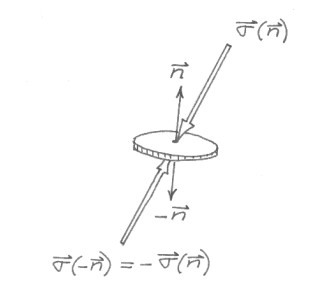
\includegraphics[scale=.8]{eq4.jpg}
\caption{Illustration of Equation 4}
\label{fig:Ill_of_eq4}
\end{figure}

where $\overrightarrow{G}$ is the body force per unit mass. When we let $\delta h$ approach zero, so that the two faces of the disc are brought toward coincidence in space, the inertial term on the left and the body force term on the right become arbitrarily small compared with the two surface force terms, and equation \ref{e4} follows immediately.

\begin{figure}[h!]
\centering
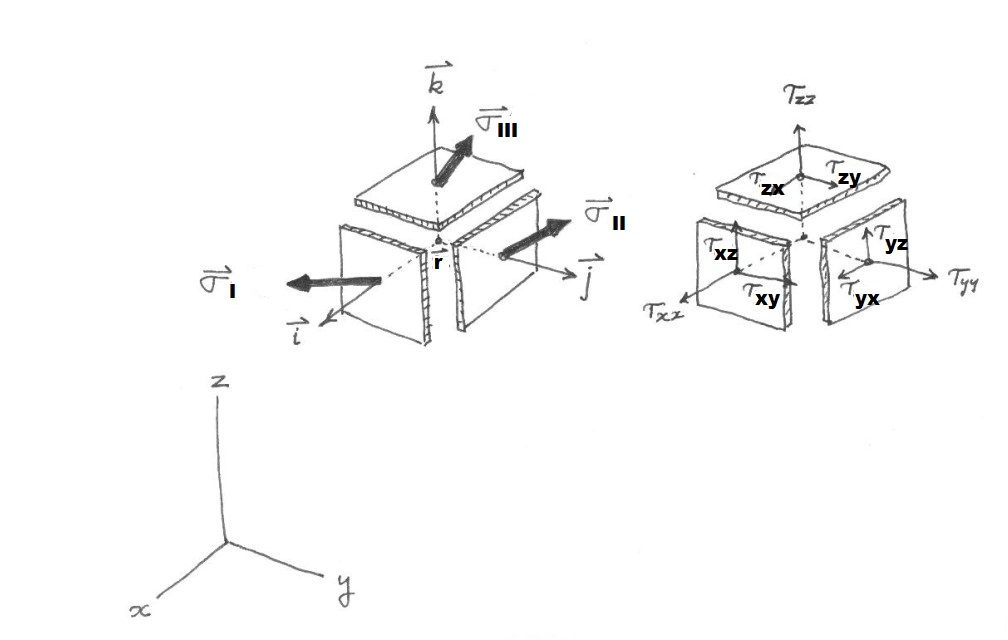
\includegraphics[scale=.6]{Reference Stresses at a point in continuum.jpg}
\caption{Reference Stresses at a point in continuum}
\label{fig:ref_strss_at_p_contnm}
\end{figure}

Newton's law also implies that the stress has a more profound attribute which leads to the concept of the stress tensor. The stress at a given point depends on the orientation of the surface element on which it acts. Let us take as "reference stresses," at a given point $\overrightarrow{r}$ and a given instant t, the values of the stresses which are exerted on a surface oriented in the positive x-direction, a surface oriented in the positive y-direction, and a surface oriented in the positive z-direction (Figure \ref{fig:ref_strss_at_p_contnm}). We can write these three "reference stresses," which of course are vectors, in terms of their components as (respectively)

\begin{equation}
\begin{split}
\bar{\sigma}_{\text{\tiny{I}}} &= \tau_{xx}\overrightarrow{i} + \tau_{xy}\overrightarrow{j} + \tau_{xz} \overrightarrow{k}\\
\bar{\sigma}_{\text{\tiny{II}}} &= \tau_{yx}\overrightarrow{i} + \tau_{yy}\overrightarrow{j} + \tau_{yz} \overrightarrow{k}\\
\bar{\sigma}_{\text{\tiny{III}}} &= \tau_{zx}\overrightarrow{i} + \tau_{zy}\overrightarrow{j} + \tau_{zz} \overrightarrow{k}\\
\end{split} \label{e6}
\end{equation}

Thus, $\tau_{xx} , \tau_{xy} \text{ and } \tau_{xz}$ represent the x, y, and z components of the stress acting on the surface whose outward normal is oriented in the positive x-direction, etc. (Figure \ref{fig:ref_strss_at_p_contnm}). The first subscript on ij indicates the outward normal of the surface on which it acts, and the second  identifies the direction of the stress. In (\ref{e6}) the ij' s are of course functions of position x, y, z, and time t, and the reference stresses themselves also depend on x, y, z, and t; we have simply not indicated this dependence.

We shall now show, again by using Newton's law, that the stress on a surface having any orientation $\overrightarrow{n}$ at the point $\overrightarrow{r}$ can be expressed in terms of the reference stresses $\bar{\sigma}_{\text{\tiny{I}}},\bar{\sigma}_{\text{\tiny{II}}},\bar{\sigma}_{\text{\tiny{III}}}$ or, more specifically, in terms of their nine components
$\tau_{xx}, \tau_{xy},...,\tau_{zz}$.

\begin{figure}[h!]
\centering
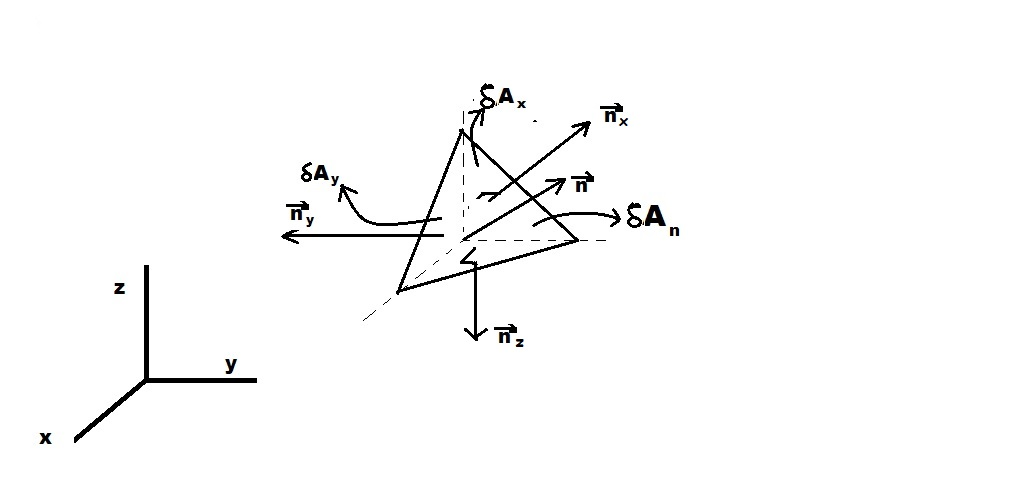
\includegraphics[scale=.6]{Tetrahedron shaped fluid particle.jpg}
\caption{Tetrahedron-Shaped fluid particle at (x,y,z)}
\label{fig:tet_shpd_partcl}
\end{figure}

Consider a fluid particle which at time t has the shape of a small tetrahedron centered at x, y, z. One of its four faces has an area A and an arbitrary outward normal $\overrightarrow{n}$ , as shown in Figure \ref{fig:tet_shpd_partcl}, and the other three faces have outward normals in the negative x, y and z directions, respectively. The areas of the three orthogonal faces are related to $\delta A$ by

\begin{equation}
\begin{split}
\delta A_{x} &= \cos(\theta_{nx})\delta A = n_{x} \delta A\\
\delta A_{y} &= \cos(\theta_{ny})\delta A = n_{y} \delta A\\
\delta A_{z} &= \cos(\theta_{nz})\delta A = n_{z} \delta A\\  \label{e7}
\end{split}
\end{equation}

where $\delta A_x$ represents the area of the surface whose outward normal is in the negative x-direction, $\theta_{nx}$ is the angle between $\overrightarrow{n}$ and the x-axis and $n_x$ is the x-component of $\overrightarrow{n}$, and so on.

Consider what Newton's law tells us about the forces acting on the tetrahedron as we let it shrink in size toward the point $\overrightarrow{r}$ around which it is centered. Since the ratio of the mass of the tetrahedron to the area of any one of its faces is proportional to the length of any one of the sides, both the mass times acceleration and the body force become arbitrarily small compared with the surface force as the tetrahedron is shrunk to a point. Hence, in the limit as the tetrahedron is shrunk to a point, the surface forces on the four faces must balance, that is,

\begin{equation}
\bar{\sigma}_{n}\delta A + \bar{\sigma}_{\text{\tiny{I}}}(-\overrightarrow{n}_{\text{\tiny{I}}})\delta A_{x} + \bar{\sigma}_{\text{\tiny{II}}}(-\overrightarrow{n}_{\text{\tiny{II}}})\delta A_{y} + \bar{\sigma}_{\text{\tiny{III}}}(-\overrightarrow{n}_{\text{\tiny{III}}})\delta A_{z} = 0 \label{e8}
\end{equation}

Now we know from (4) that the stress on a surface pointing in the $-\overrightarrow{i}$ direction is the negative of the stress on a surface in the $+\overrightarrow{i}$ direction, etc. Using this result and (\ref{e7}) for theareas, (\ref{e8}) becomes

\begin{equation}
\bar{\sigma}_{n}\delta A = \bar{\sigma}_{\text{\tiny{I}}}n_{x} + \bar{\sigma}_{\text{\tiny{II}}}n_{y} + \bar{\sigma}_{\text{\tiny{III}}}n_{z} \label{e9}
\end{equation}

Alternatively, if we use (\ref{e6}) to write the reference stresses in terms of their components, we obtain the components of $\bar{\sigma}_{n}$ as

\begin{align*}
\bar{\sigma}_{n}\delta A &= (\tau_{xx}\overrightarrow{i} + \tau_{xy}\overrightarrow{j} + \tau_{xz} \overrightarrow{k})n_{x} + (\tau_{yx}\overrightarrow{i} + \tau_{yy}\overrightarrow{j} + \tau_{yz} \overrightarrow{k})n_{y} + (\tau_{zx}\overrightarrow{i} + \tau_{zy}\overrightarrow{j} + \tau_{zz} \overrightarrow{k})n_{z}\\
						 &= (\tau_{xx}n_{x} + \tau_{yx}n_{y} + \tau_{zx})\overrightarrow{i} + (\tau_{xy}n_{x} + \tau_{yy}n_{y} + \tau_{zy})\overrightarrow{j} + (\tau_{xz}n_{x} + \tau_{yz}n_{y} + \tau_{zz})\overrightarrow{k}
\end{align*}

\begin{equation}
\begin{split}
\bar{\sigma}_{nx} &= \tau_{xx}n_{x} + \tau_{yx}n_{y} + \tau_{zx}n_{z}\\
\bar{\sigma}_{ny} &= \tau_{xy}n_{x} + \tau_{yy}n_{y} + \tau_{zy}n_{z}\\
\bar{\sigma}_{nz} &= \tau_{xz}n_{x} + \tau_{yz}n_{y} + \tau_{zz}n_{z}\\ \label{e10}
\end{split}
\end{equation}

Thus the stress $\bar{\sigma}_{n}$ acting at $\overrightarrow{r},t$ on a surface with any arbitrary orientation $\overrightarrow{n}$ can be expressed in terms of the nine reference stress components

$$\begin{bmatrix}
\tau_{xx} & \tau_{yx} & \tau_{zx} \\
\tau_{xy} & \tau_{yy} & \tau_{zy} \\
\tau_{xz} & \tau_{yz} & \tau_{zz} \\
\end{bmatrix}$$

These nine quantities, each of which depends on position and time, are the stress tensor components. Once the stress tensor components are known at a given point, one can compute the surface stress acting on any surface drawn through that point: one simply determines the components of the outward unit normal $\overrightarrow{n}$ of the surface involved, and uses (\ref{e10}).

Equation (\ref{e10}) can be written more succinctly in conventional tensor notation. In this notation (\ref{e10}) reads simply

\begin{equation}
\sigma_{i}(\overrightarrow{x},t,\overrightarrow{n}) = \tau_{ji}(\overrightarrow{x},t)n_{j} \label{e11}
\end{equation}

The importance of the stress tensor concept in continuum theory is this: It allows us to describe the state of stress in a continuum in terms of quantities that depend on position and time, but not on the orientation of the surface on which the stress acts. Admittedly, nine such quantities are needed (actually only six are independent, as we shall see shortly). Still, it is far easier to deal with them than with a single quantity which, at any given position and time, has a doubly infinite set of values corresponding to different surface
orientations $\overrightarrow{n}$.

Physically, the stress tensor represents the nine components of the three reference stresses at the point $\overrightarrow{r}$ and time t in question. The reference stresses are by custom chosen as the stresses on the three surface elements that have outward normals in the direction of the positive axes of the coordinate system being used. Thus in our Cartesian coordinates, the reference stresses are the stresses on the surfaces pointing in the positive x, y, and z directions, and the stress tensor is made up of the nine components of these three stresses, $\tau_{ji}$ being the j-component of the stress on the surface whose normal points in the i-direction.

The front face $\Delta$ABC belongs to the plane which is describes by the following formula

$$(\overrightarrow{n},\overrightarrow{x}-\overrightarrow{x_{0}}) = h, \text{Here h is very small due to fact that the plane is very close to origin}$$

The areas of the faces of the tetrahedron are S, $S_1$, $S_2$ and $S_3$ for $\Delta ABC$, $\Delta OBC$, $\Delta AOC$ and $|delta ABO$, respectively

\begin{figure}[h!]
\centering
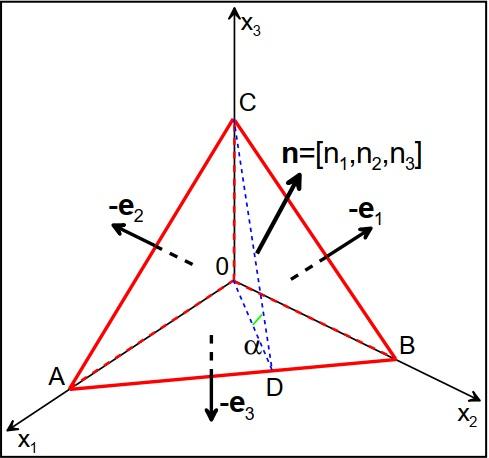
\includegraphics[scale=.4]{Constitutive Property.jpg}
\caption{Constitutive Property}
\label{fig:Consti_prop}
\end{figure}

$$S\backsim O(h^{2})$$ 

Moreover, the following relations hold for j = 1,2,3:

$$S_{j} = S\cos(\angle(\overrightarrow{n},\overrightarrow{e_{j}})) = S\cdot (\overrightarrow{n},\overrightarrow{e_{j}}) = Sn_{j}$$

The volume of the tetrahedron is $V_{\Omega}\backsim O(h^{3})$

The momentum principle for the fluid contained inside the tetrahedron volume reads

$$\frac{d}{dt}\int_{\Omega}\rho vdx = F_{vol} + F_{surf}$$

We need to calculate the total surface force $F_{surf}$ . We have\footnote{we want to approximate say $\sigma(\overrightarrow{x},\overrightarrow{n})$ as $\sigma$ at 0 and some other terms of O(h). I can't figure out why O(h) by mathematical reasoning. What are the assumptions? One way thinking is since h is very small and the stress was acting on plane ABC, so if we write $\overrightarrow{x} = hl\overrightarrow{i} + hm\overrightarrow{j} + hn\overrightarrow{k}$ where l,m,n are direction cosines of plane ABC. So $\sigma(\overrightarrow{x},\overrightarrow{n}) = \sigma(0+h,\overrightarrow{n}) = \sigma(0,\overrightarrow{n}) + O(h).$}

\begin{align*}
\text{on } \Delta ABC: \quad & \sigma(\overrightarrow{x},\overrightarrow{n}) = \sigma(0,n) + O(h)\\
							& F_{\text{surf}}^{\Delta ABC} = S\sigma(0,n) + O(h^{3}) 
\end{align*}

\begin{align*}
\text{on } \Delta OBC: \quad & \sigma(\overrightarrow{x},-\overrightarrow{e_{1}}) = -\sigma(\overrightarrow{x},\overrightarrow{e_{1}})= -\sigma(0,\overrightarrow{e_{1}}) + O(h)\\
							& F_{\text{surf}}^{\Delta OBC} = -S_{1}\sigma(0,\overrightarrow{e_{1}}) + O(h^{3}) = -Sn_{1}\sigma(0,n_{1}) + O(h^{3})
\end{align*}

\begin{align*}
\text{on } \Delta AOC: \quad & \sigma(\overrightarrow{x},-\overrightarrow{e_{2}}) = -\sigma(\overrightarrow{x},\overrightarrow{e_{2}})= -\sigma(0,\overrightarrow{e_{2}}) + O(h)\\
							& F_{\text{surf}}^{\Delta AOC} = S_{2}\sigma(0,\overrightarrow{e_{2}}) + O(h^{3})  = -Sn_{2}\sigma(0,n_{2}) + O(h^{3})
\end{align*}

\begin{align*}
\text{on } \Delta AOB: \quad & \sigma(\overrightarrow{x},-\overrightarrow{e_{3}}) = -\sigma(\overrightarrow{x},\overrightarrow{e_{3}})= -\sigma(0,\overrightarrow{e_{3}}) + O(h)\\
							& F_{\text{surf}}^{\Delta AOB} = -S_{3}\sigma(0,\overrightarrow{e_{3}}) + O(h^{3}) = -Sn_{3}\sigma(0,n_{3}) + O(h^{3})
\end{align*}

When the above formulas are inserted to the equation of motion we get

$$\frac{d}{dt}\int_{\Omega}\rho vdx = F_{vol} + S[\sigma(0,\overrightarrow{n}) - n_{j}\sigma(0,\overrightarrow{n})] + O(h^{3})$$

When $h\to 0$ the above equation reduces to

$$\sigma(0,\overrightarrow{n}) - n_{j}\sigma(0,\overrightarrow{n}) = 0$$

In general case, the vertex O is not the origin of the coordinate system and the field of stress is time dependent.

Here, we can write  $\sigma(t,\overrightarrow{x},\overrightarrow{n}) = n_{j}\sigma(t,\overrightarrow{x},\overrightarrow{e_{j}})$

In the planes oriented perpendicularly to the vectors e1, e2 or e3, the stress vector can be
written as $\sigma(t,\overrightarrow{x},\overrightarrow{e_{j}}) = \sigma_{ij}(t,\overrightarrow{x})\overrightarrow{e_{i}}$

Thus, the general formula for the stress vector takes the form 

$$\sigma(t,\overrightarrow{x},\overrightarrow{n}) = n_{j}\sigma(t,\overrightarrow{x},\overrightarrow{e_{j}}) = \sigma_{ij}(t,\overrightarrow{x})n_{j}\overrightarrow{e_{i}} = \rotatebox[origin=c]{90}{\textbf{[I]}}(t,\overrightarrow{x})\overrightarrow{n}$$

We have introduced the matrix $\rotatebox[origin=c]{90}{\textbf{[I]}}$ which represents the stress tensor. The stress tensor depends on time and space coordinates, i.e., we actually have the tensor field.

the stress tensor $\rotatebox[origin=c]{90}{\textbf{[I]}}$ can be viewed as the linear mapping (parameterized by t and x) between vectors in 3-dimensional Euclidean space

$$\rotatebox[origin=c]{90}{\textbf{[I]}}:E^{3} \rotatebox[origin=c]{180}{$\in$} \overrightarrow{w} = w_{j}\overrightarrow{e_{j}}\to \sigma_{ij}w_{j}\overrightarrow{e_{i}}\in E^{3}$$

In particular,

$$\rotatebox[origin=c]{90}{\textbf{[I]}}(\overrightarrow{n})\equiv \rotatebox[origin=c]{90}{\textbf{[I]}}\overrightarrow{n} = \sigma_{ij}n_{j}\overrightarrow{e_{i}} = \overrightarrow{\sigma}$$

i.e., the action of $\rotatebox[origin=c]{90}{\textbf{[I]}}$ on the normal vector $\overrightarrow{n}$ at some point of the fluid surface yields the stress vector $\overrightarrow{\sigma}$ at this point

It is often necessary to calculate the normal and tangent stress components at the point of
some surface.

Normal component is equal

$$\overrightarrow{\sigma_{n}} = (\overrightarrow{n}\cdot\rotatebox[origin=c]{90}{\textbf{[I]}}\overrightarrow{n})\overrightarrow{n} \equiv (\overrightarrow{n},\rotatebox[origin=c]{90}{\textbf{[I]}}\overrightarrow{n})\overrightarrow{n}$$

where $(\overrightarrow{n},\rotatebox[origin=c]{90}{\textbf{[I]}}\overrightarrow{n})$ is a inner product.

\begin{align*}
(\overrightarrow{n},\rotatebox[origin=c]{90}{\textbf{[I]}}\overrightarrow{n})\overrightarrow{n} &= (n_{m}\overrightarrow{e_{m}},\sigma_{kl}n_{k}\overrightarrow{e_{l}})n_{i}\overrightarrow{e_{i}}\\
																								&= n_{k}n_{m}\sigma_{kl}(\overrightarrow{e_{l}},\overrightarrow{e_{m}})n_{i}\overrightarrow{e_{i}}\\
																								&= (n_{k}n_{m}\sigma_{kl}\delta_{lm})n_{i}\overrightarrow{e_{i}}\\
																								&= (n_{k}n_{m}\sigma_{km})n_{i}\overrightarrow{e_{i}}
\end{align*}

Tangent component can be expressed as 

$$\overrightarrow{\sigma_{t}} = \overrightarrow{\sigma} - \sigma_{n}\overrightarrow{n} = \sigma_{ij}n_{j}\overrightarrow{e_{i}} - (\sigma_{km}n_{k}n_{m})n_{i}\overrightarrow{e_{i}} = [\sigma_{ij}n_{j} - (\sigma_{km}n_{k}n_{m})n_{i}]\overrightarrow{e_{i}}$$

or, equivalently as

$$\overrightarrow{\sigma_{t}} = \overrightarrow{n}\times(\overrightarrow{\sigma}\times \overrightarrow{n})$$

Indeed, using the identity $\overrightarrow{a}\times(\overrightarrow{b}\times \overrightarrow{c}) = (\overrightarrow{a},\overrightarrow{c})\overrightarrow{b} - (\overrightarrow{a},\overrightarrow{b})\overrightarrow{c}$

for $\overrightarrow{a} = \overrightarrow{n}, \overrightarrow{b} = \overrightarrow{\sigma}, \overrightarrow{c} = \overrightarrow{n}$ we obtain

$$\overrightarrow{\sigma_{t}} = \overrightarrow{n}\times(\overrightarrow{\sigma}\times \overrightarrow{n}) = (\overrightarrow{n},\overrightarrow{n})\overrightarrow{\sigma} - (\overrightarrow{n},\overrightarrow{\sigma})\overrightarrow{n} = \overrightarrow{\sigma} - \overrightarrow{\sigma_{n}}$$

$\overrightarrow{n}$ is a unit vector, so $(\overrightarrow{n},\overrightarrow{n}) = 1$ 


\section*{Constitutive Relation}

The constitutive relation for the (simple) fluids is the relation between stress tensor $\rotatebox[origin=c]{90}{\textbf{[I]}}$ and the deformation rate tensor $\mathit{D}$. This relation should be postulated in a form which is frame invariant and such that the stress tensor is symmetric.

There are two facts:

\begin{itemize}
\item[•] The velocity gradient $\nabla\mathcal{V}$ can be decomposed into two parts: the symmetric part $\mathit{D}$ called the deformation rate tensor and the skew-symmetric part $\mathit{R}$ called the (rigid) rotation tensor.

$$\nabla\mathcal{V} = \mathbf{D} + \mathbf{R}$$

\item[•] Tensor $\mathbf{D}$ can be expressed as the sum of the spherical part $\mathbf{D}_{SPH}$ and the deviatoric part $\mathbf{D}_{DEV}$

$$\mathbf{D} = \mathbf{D}_{SPH} + \mathbf{D}_{DEV}$$
\end{itemize}


Where 

$$\mathbf{D}_{SPH} = \frac{1}{3}tr\mathbf{D}\cdot\mathbf{I} = \frac{1}{3}(\nabla\cdot \mathcal{V})\mathbf{I}$$

$$\mathbf{D}_{DEV} = \mathbf{D}-\frac{1}{3} div \mathcal{V}\cdot \mathbf{I}\Rightarrow (D_{DEV})_{ij} = \frac{1}{2}\bigg(\frac{\partial \mathcal{V}_{i}}{\partial x_{j}} + \frac{\partial \mathcal{V}_{j}}{\partial x_{i}}\bigg)-\frac{1}{3}\frac{\partial \mathcal{V}_{k}}{\partial x_{k}}\delta_{ij}$$

The general constitutive relation for a (simple) fluid can be written in the form of the matrix
“polynomial”

\section*{Symmetry of Stress Tensor}

One further piece of information emerges from applying Newton's law to an infinitesimal fluid particle. This is that the stress tensor is in most cases symmetric, that is, $\tau_{ji} = \tau_{ij}, \text{ for } i\neq j$.

\begin{figure}[h!]
\centering
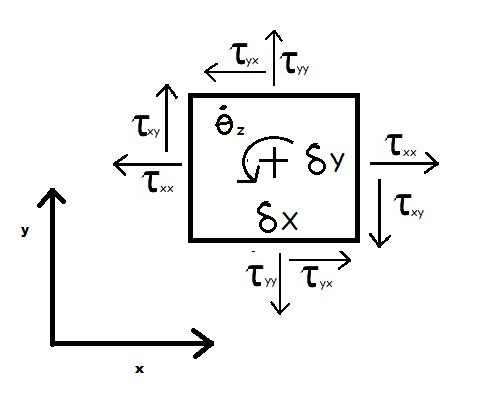
\includegraphics[scale=.8]{Illustration of the reason for the stress tensor's symmetry.jpg}
\caption{Illustration of the reason for the stress tensor's symmetry}
\label{fig:Illus_rsn_strss_tensr_symm}
\end{figure}


The proof follows from considering the angular acceleration of a little fluid particle at x, y, z. For convenience, we let it be shaped like a little cube with infinitesimal sides $\delta x, \delta y,\text{ and }\delta z$ (Figure \ref{fig:Illus_rsn_strss_tensr_symm}). Since we shall be taking the limit where $\delta x, \delta y,\delta z \to 0$, where the fluid particle is reduced to a point, we can safely assume that the values of the density, velocity, stress tensor components, etc. are almost uniform throughout the cube. What is more, if the cube rotates by an infinitesimal amount, it does so almost as a solid body (i.e. at essentially zero angular distortion), since in the limit $\delta x, \delta y,\delta z \to 0$ a finite angular distortion would require infinite shear in a viscous fluid. If the cube has an angular velocity $\dot{\theta_{z}}$ in the z-direction, say, and rotates like a solid body, we can derive from Newton's law written in angular momentum form for a material volume, that at any given instant its angular velocity increases according to 

$$I_{z}\frac{\text{d}\dot{\theta_{z}}}{\text{d}t} = T_{z}$$

where

$$I_{z} = \int_{-\frac{\delta x}{2}}^{\frac{\delta x}{2}}\int_{-\frac{\delta y}{2}}^{\frac{\delta y}{2}}\int_{-\frac{\delta z}{2}}^{\frac{\delta z}{2}}\rho(\bar{x}^{2}+\bar{y}^{2})\text{d}\bar{x}\text{d}\bar{y}\text{d}\bar{z} = \frac{\rho[(\delta x)^2 + (\delta y)^2]}{12}\delta x\delta y \delta z$$

is the moment of inertia of the cube and $T_z$ is the net torque acting on the cube, relative to
an axis running through the center of the cube parallel to the z-axis. Equation (13) is obtained by writing the cube’s angular velocity as $v_{\theta} = \bar{\theta}(t)r$, where $r^2 = \bar{x}^2 + \bar{y}^2$, $\bar{x}$ and $\bar{y}$ being the Cartesian coordinates fixed in the rotating cube.

The torque $T_{z}$ is obtained by considering the stresses acting on the cube (Figure \ref{fig:Illus_rsn_strss_tensr_symm}). On the face with $\overrightarrow{n} = \overrightarrow{i}$, for example, there is by definition a stress $\tau_{xx}$ in the positive x-direction and a stress $\tau_{xy}$ in the positive y-direction. On the face with $\overrightarrow{n} = -\overrightarrow{i}$, the corresponding stresses have the same magnitudes but opposite directions.


The net torque about an axis through the cube's center, parallel to the z-axis, is caused by
the shear forces (the pressure forces act through the cube’s center) and by any volumetric
torque exerted by the external body force field. A body force field like gravity acts through
the cube's center of mass and exerts no torque about that point. Let us assume for the sake
of generality, however, that the external body force may exert a torque $\overrightarrow{t}$ per unit volume at the particle's location. The net torque in the z-direction around the particle's center would then be

$$T_{z} = 2\tau_{yx}\frac{\delta y}{2}\delta x\delta z - 2\tau_{xy}\frac{\delta x}{2}\delta y\delta z + t_{z}\delta x\delta y\delta z = (\tau_{yx}-\tau_{xy}+t_{z})\delta x\delta y\delta z$$

\begin{equation}
\begin{split}
\frac{\rho[(\delta x)^2 + (\delta y)^2]}{12}\delta x\delta y \delta z\frac{\text{d}\dot{\theta_{z}}}{\text{d}t} &= (\tau_{yx}-\tau_{xy}+t_{z})\delta x\delta y\delta z\\
\frac{\rho[(\delta x)^2 + (\delta y)^2]}{12}\frac{\text{d}\dot{\theta_{z}}}{\text{d}t} &= \tau_{yx}-\tau_{xy}+t_{z} \label{e12}
\end{split}
\end{equation}

As we approach a point in the fluid by letting $\delta x, \delta y \to 0$, this reduces to

$$\tau_{xy} = \tau_{yx} + t_{z}$$

or, more generally, the result that the off-diagonal stress tensor components must satisfy

\begin{equation}
\tau_{ij} = \tau_{ji} + t_{k} \label{e13}
\end{equation}

where i, j, k form a right-hand triad (e.g. in Cartesian coordinates they are in the order x,
y, z, or y, z, x, or z, x, y).

Volumetric body torque can exist in magnetic fluids ,we shall assume that volumetric body torque is absent, in which case (\ref{e13}) shows that the off-diagonal or shear terms in the stress tensor are symmetric,

\begin{equation}
\tau_{ij} = \tau_{ji} \text{ for } i \neq j \label{e14}
\end{equation}

This means that three of the nine components of the stress tensor can be derived from the remaining ones; that is, the stress tensor has only six independent components.

\section*{Equation of Motion in Terms of the Stress Tensor}

\begin{figure}[h!]
\centering
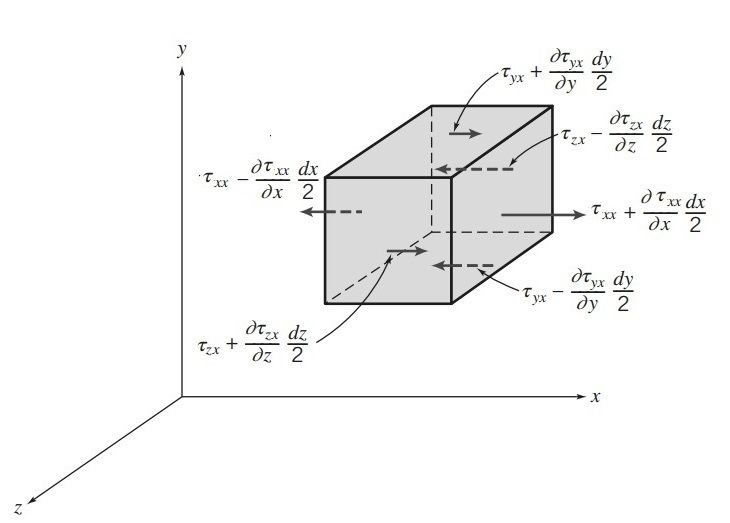
\includegraphics[scale=.9]{x-direction surface stresses acting on a fluid particle.jpg}
\caption{x-direction surface stresses acting on a fluid particle}
\label{fig:x_dir_surf_stress}
\end{figure}

A general equation of motion in differential form may be derived by applying Newton's law to a small but finite fluid particle. Consider again a particle which at time t has the shape of a cube centered about (x, y, z) as in Figure \ref{fig:x_dir_surf_stress}, with sides $\delta x, \delta y, \text{ and } \delta z$ parallel to the x, y, and z axes at time t. Although the sides are small, they are not zero and the components of the stress tensor will have slightly different values on the faces of the cube than at the center of the cube. For example, if the stress tensor components $\tau_{ij}$ are specified at (x, y, z), the center of the cube, then their values will be

$$\tau_{ij} + \frac{\partial \tau_{ij}}{\partial x}\frac{\delta x}{2}$$

at the face whose outward normal is in the positive x-direction, and

$$\tau_{ij} - \frac{\partial \tau_{ij}}{\partial x}\frac{\delta x}{2}$$

at the opposite face.

Figure \ref{fig:x_dir_surf_stress} shows all those stresses which act on the cube in the x-direction, expressed in terms of the stress tensor. The arrows indicate the directions of the stresses for positive values of $\tau_{ij}$. The net x-component of surface force on the cube is obtained by multiplying the stresses by the areas on which they act and summing:

$$\bigg(\frac{\partial \tau_{xx}}{\partial x} + \frac{\partial \tau_{yx}}{\partial y} + \frac{\partial \tau_{zx}}{\partial z}\bigg)\delta x\delta y\delta z$$

Since $\delta x \delta y \delta z$ is the particle's volume, we identify the quantity within the brackets as the
net x-component of surface force per unit volume at a point in a fluid. The expressions for
the y and z components are similar, except that the second subscript x is replaced by y and z,
respectively.

The equation of motion can now be written down directly for the cubical fluid particle in Figure \ref{fig:x_dir_surf_stress}. The x-component of the equation states that the mass times the acceleration equals the net surface force plus the body force acting on the particle:

\begin{align*}
\rho \delta x\delta y\delta z \frac{Dv_{x}}{Dt} &= \bigg(\frac{\partial \tau_{xx}}{\partial x} + \frac{\partial \tau_{yx}}{\partial y} + \frac{\partial \tau_{zx}}{\partial z}\bigg)\delta x\delta y\delta z + \rho G_{x}\delta x\delta y\delta z
\end{align*}

Here, $\frac{D}{Dt}$ represents the substantial derivative, which is defined elsewhere, and $G_x$ is the x-component of the external body force per unit mass. This yields

\begin{equation}\label{e15a} 
\rho \frac{Dv_{x}}{Dt} = \bigg(\frac{\partial \tau_{xx}}{\partial x} + \frac{\partial \tau_{yx}}{\partial y} + \frac{\partial \tau_{zx}}{\partial z}\bigg) + \rho G_{x}\tag{15a}
\end{equation}

For the y and z components we obtain similarly

\begin{equation}\label{e15b} 
\rho \frac{Dv_{y}}{Dt} = \bigg(\frac{\partial \tau_{xy}}{\partial x} + \frac{\partial \tau_{yy}}{\partial y} + \frac{\partial \tau_{zy}}{\partial z}\bigg) + \rho G_{y}\tag{15b}
\end{equation}

\begin{equation}\label{e15c} 
\rho \frac{Dv_{z}}{Dt} = \bigg(\frac{\partial \tau_{xz}}{\partial x} + \frac{\partial \tau_{yz}}{\partial y} + \frac{\partial \tau_{zz}}{\partial z}\bigg) \rho G_{z}\tag{15c}
\end{equation}

or, more succinctly,

\begin{equation}
\rho \frac{Dv_{i}}{Dt} = \frac{\partial \tau_{ij}}{\partial x_{j}} + \rho G_{i} \label{e15}
\end{equation}

where a summation over j=x, y, and z is implied. Equation (\ref{e15}) states that at a given point and time, the mass per unit volume times the acceleration in the i-direction (the left-hand
term) equals the the net surface force per unit volume in the i-direction (the first term on the
right) plus the body force per unit volume in the i-direction (the second term on the right). The equation applies quite generally to any continuous distribution of matter, whether fluid or solid, and is not based on any assumption other than that the continuum hypothesis applies. Equation (20) is, however, incomplete as it stands. To complete it, one must specify the stress tensor components and the body force components, just as one must define the forces acting on a solid particle before one can derive its motion. The specification of the body force is straightforward. In a gravitational field, for example, the force per unit mass is well known and is of the same form for all substances. The form of the stress tensor is different for different classes of materials.

\section*{Stress Tensor for Newtonian Fluids}

There remains the task of specifying the relationship between the stress tensor components and the flow or deformation field. The simplest model of a solid continuum is the well-known elastic one, where stresses and strains are linearly related. The defining attribute of a simple fluid, however, is that it keeps deforming, or straining, as long as any shear stress, no matter how small, is applied to it. Obviously, no unique relation can exist between the shear stresses and the shear strains if strain can increase indefinitely at constant shear. It is observed, however, that a fluid tends to resist the rate of deformation: the higher the applied shear stress, the faster the rate of shear deformation. In many fluids the relation between stress and rate of strain in a fluid particle is linear under normal conditions.

The Newtonian model of fluid response is based on three assumptions:
\begin{itemize}
\item[•] shear stress is proportional to the rate of shear strain in a fluid particle
\item[•] shear stress is zero when the rate of shear strain is zero
\item[•] the stress to rate-of-strain relation is isotropic—that is, there is no preferred orientation in the fluid.
\end{itemize}

A Newtonian fluid is the simplest type of viscous fluid, just like an elastic solid (where stresses are proportional to strains) is the simplest type of deformable solid.

To implement the Newtonian assumptions we consider first a typical shear term in the tensor, e.g $\tau_{xy}$ . Figure \ref{fig:shr_defrmtn_fl_prtcl}  depicts the deformation of a fluid particle as it moves between time t and time t+dt. In this interval the shear stress $\tau_{xy}$ produces in the fluid particle an incremental angular strain $\text{d}\gamma_{xy}$

\begin{figure}[h!]
\centering
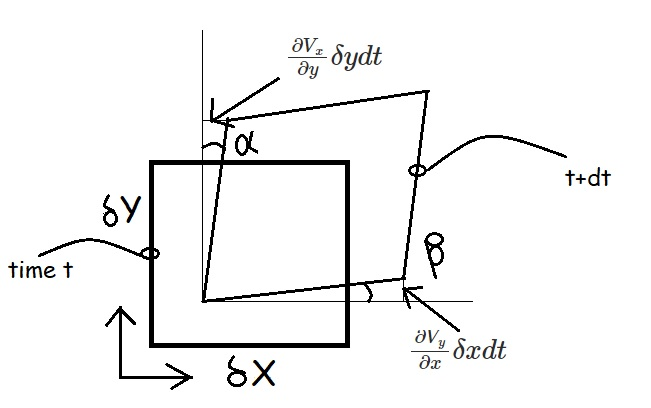
\includegraphics[scale=.5]{shear deformation in a fluid particle.jpg}
\caption{Shear deformation in a fluid particle}
\label{fig:shr_defrmtn_fl_prtcl}
\end{figure}

For small angle $\alpha$ \& $\beta$ we can write 

$$\tan(\alpha) + \tan(\beta) = \alpha + \beta = d\gamma_{xy} = \frac{\frac{\partial V_{x}}{\partial y}\delta y dt}{\delta y} + \frac{\frac{\partial V_{y}}{\partial x}\delta x dt}{\delta x} =  \frac{\partial V_{x}}{\partial y} + \frac{\partial V_{y}}{\partial x}$$

The rate of angular strain in the fluid particle as seen by an observer sitting on it is therefore

$$\frac{D\gamma_{xy}}{Dt} = \frac{\partial V_{x}}{\partial y} + \frac{\partial V_{y}}{\partial x}$$

According to newtonian assumption 

\begin{equation} \label{16a}
\tau_{xy} = \mu \frac{D\gamma_{xy}}{Dt} = \mu \bigg(\frac{\partial V_{x}}{\partial y} + \frac{\partial V_{y}}{\partial x}\bigg) \tag{16a}
\end{equation}

where the coefficient of proportionality $\mu$ is called the shear, or ``ordinary", viscosity
coefficient, and is a property of the fluid. Similarly

\begin{equation} \label{16b}
\tau_{xz} = \mu \frac{D\gamma_{xz}}{Dt} = \mu \bigg(\frac{\partial V_{x}}{\partial z} + \frac{\partial V_{z}}{\partial x}\bigg) \tag{16b}
\end{equation}

\begin{equation} \label{16c}
\tau_{yz} = \mu \frac{D\gamma_{yz}}{Dt} = \mu \bigg(\frac{\partial V_{y}}{\partial z} + \frac{\partial V_{z}}{\partial y}\bigg) \tag{16c}
\end{equation}

or in general,

\begin{equation}
\tau_{ij} = \mu\bigg(\frac{\partial V_{i}}{\partial x^{j}} + \frac{\partial V_{j}}{\partial x^{i}}\bigg)
\end{equation}

The coefficient of proportionality is the same in all three shear stresses because a
Newtonian fluid is isotropic.

Next Let's consider a typical normal stress, that is, one of the stress tensor's diagonal
terms, say $\tau_{xx}$ . The derivation of such a term's form is not as simple as that of the shear terms, but can nevertheless be done in fairly physical terms by noting that linear and shear deformations generally occur hand in hand. The trick is to find how the linear stresses and deformations are related to the shear stresses and deformations.


Consider a small fluid particle which at time t is a small cube with sides of length h
parallel to the x, y and z axes. We will again be considering the limit of a particle "at a
point", that is, the limit h $\to$ 0. At time t , its corner A is at (x, y, z). Between t and t+dt, it moves and deforms as in Figure \ref{fig:Reln_betn_lin_&_shr_dfrmtn} The sides AB and AD will in general rotate by unequal
amounts. This will result in a shear deformation of the particle. The shear deformation will
cause one of the diagonals AC and BD to expand and the other to contract, that is, it will 
give rise to linear deformations in the $x^{'}$ and $y^{'}$ directions which are rotated $45^{o}$ relative to the x and y axes. 

\begin{figure}[h!]
\centering
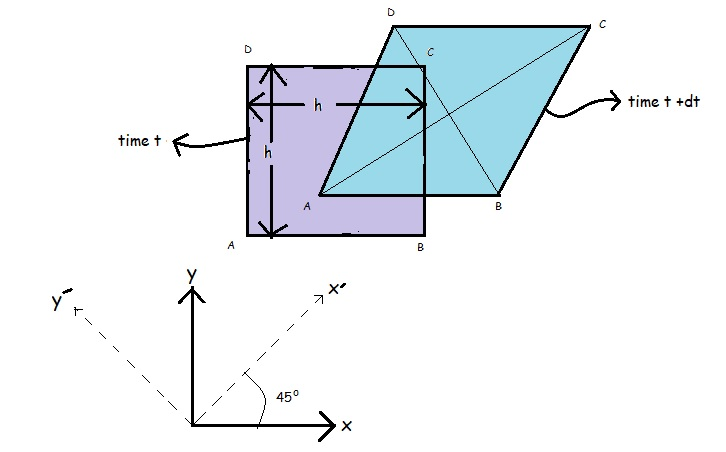
\includegraphics[scale=.9]{Relation between linear and shear deformation.jpg}
\caption{Relation between linear and shear deformation}
\label{fig:Reln_betn_lin_&_shr_dfrmtn}
\end{figure}

Now, we know the relationship between the shear stress and the rate of angular strain of the particle in the (x, y) frame. If we can connect the shear stresses in this frame and the stresses in the rotated ($x^{'}$, $y^{'}$) frame, and the shear strain rates in the (x, y) frame and the
strain rates on the ($x^{'}$, $y^{'}$) frame, we will arrive at a relation between the stresses and the strain rates in the ($x^{'}$, $y^{'}$) frame. Since the reference frames are arbitrary, the relationship between stresses and rates of strain for the ($x^{'}$, $y^{'}$) frame must be general in form.

We start by considering the forces acting on one half of the fluid particle in Figure \ref{fig:stress_on_2_1_2_particle} the triangular fluid particle ABD as shown in Figure \ref{fig:stress_on_2_1_2_particle}. Since we are considering the limit h $\to$ 0, where the ratio of volume to area vanishes, the equation of motion for the particle will reduce to the statement that the surface forces must be in balance. Figure \ref{fig:stress_on_2_1_2_particle} shows the surface forces on particle ABD, expressed in terms of the stress tensor components in the original and the rotated reference frames.

\begin{figure}[h!]
\centering
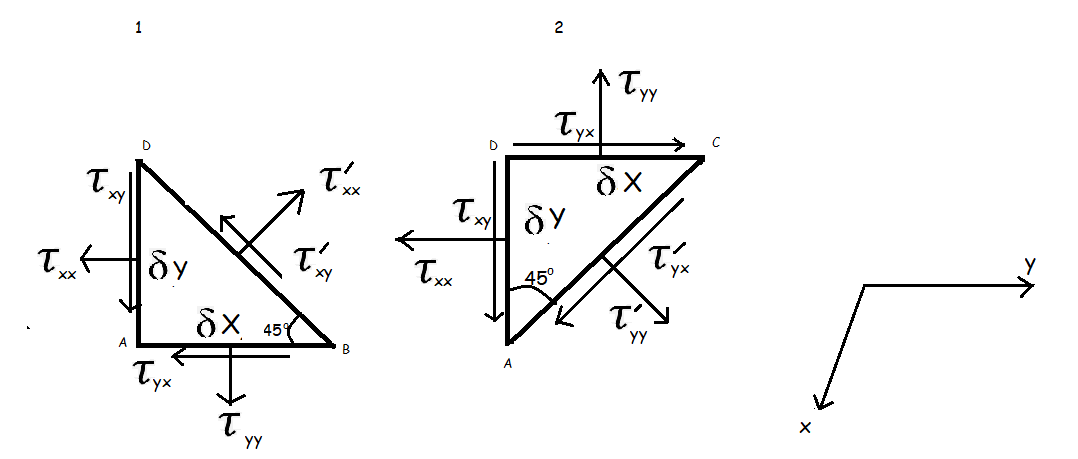
\includegraphics[scale=.6]{Stress on two halves particle.png}
\caption{Stress on two halves particle on Figure \ref{fig:Reln_betn_lin_&_shr_dfrmtn}}
\label{fig:stress_on_2_1_2_particle}
\end{figure}

A force balance in the $x^{'}$-direction gives

\begin{align*}
 & +\rotatebox[origin=c]{-30}{$\uparrow$}\sum F_{x^{'}} = 0 \\
 & \tau^{'}_{xx}\delta l - \tau_{xx}\delta {y}\cos(45^{o}) - \tau_{yy}\delta {x}\cos(45^{o}) - \tau_{xy}\delta y\cos(45^{o}) - \tau_{yx}\delta x\cos(45^{o})=0
\end{align*}

for both triangles (1) \& (2) we have, $\delta x = \delta y = \delta l\cos(45^{o})$

for $\Delta$ABD we get, 

\begin{equation} \label{e17}
\tau_{xx}^{'} = \frac{\tau_{xx}+\tau_{yy}}{2} + \tau_{yx}
\end{equation}

Similarly, a force balance in the y'-direction on the triangular particle ACD gives

\begin{align*}
& +\rotatebox[origin=c]{-120}{$\uparrow$}\sum F_{y^{'}} = 0\\
& \tau^{'}_{yy}\delta l - \tau_{xx}\delta {y}\cos(45^{o}) - \tau_{yy}\delta {x}\cos(45^{o}) + \tau_{xy}\delta y\cos(45^{o}) + \tau_{yx}\delta x\cos(45^{o})=0
\end{align*}
 
\begin{equation} \label{e18}
\begin{split}
& \tau_{yy}^{'} = \frac{\tau_{xx}+\tau_{yy}}{2} - \tau_{yx}
\end{split}
\end{equation}

Substracting (\ref{e18}) and (\ref{e17}) we obtain

\begin{equation} \label{e19}
\tau^{'}_{xx} - \tau^{'}_{yy} = 2\tau_{yx}
\end{equation}

Using the relation (16a) between the shear stress and the rate of strain, this becomes

\begin{equation}\label{e20}
\tau^{'}_{xx} - \tau^{'}_{yy} = 2\mu \frac{D\gamma_{xy}}{Dt}
\end{equation}

which relates the diagonal stress tensor terms in the ($x^{'},y^{'}$) frame to the angular strain rate in the (x, y) frame.

\begin{figure}[h!]
\centering
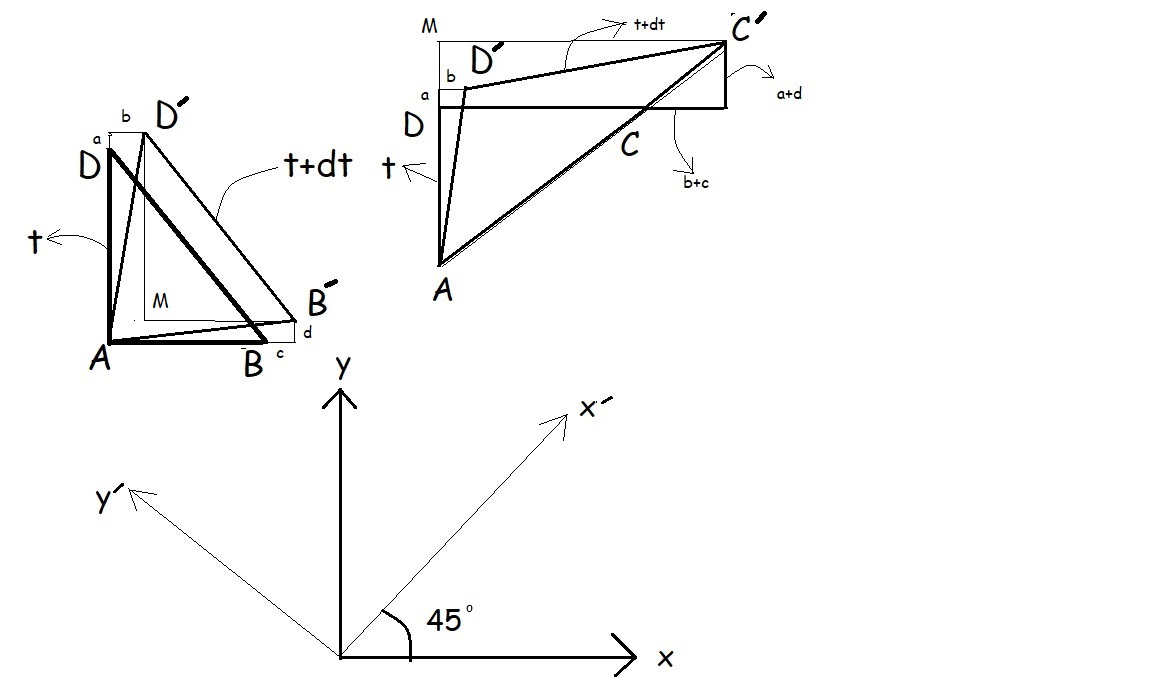
\includegraphics[scale=.43]{Deformation of triangle particle.jpg}
\caption{Deformation of triangle particle in Figure \ref{fig:stress_on_2_1_2_particle}}
\label{fig:Defrmtn_of_trngl_prtcl}
\end{figure}

To close the loop we must relate the angular strain rate in the (x, y) frame to the
strain rates in the ($x^{'},y^{'}$) frame. Figure \ref{fig:Defrmtn_of_trngl_prtcl} shows the deformations of the triangular particles ABD and ACD between t and t+dt. The deformations a, b, c, and d in the figure are related to the incremental linear strains d$\epsilon$ and angular strains d$\gamma$ in the (x, y) frame by

\begin{equation} \label{e21}
\begin{split}
d\epsilon_{x} &= \frac{c}{h}\\
d\epsilon_{y} &= \frac{a}{h}\\
d\gamma_{xy} &= \frac{b+d}{h} \text{ \{same way we derived shear}\\ 
			 &	\quad\quad\quad\quad \text{ deformation of fluid particle\}}
\end{split}
\end{equation}

Here, d$\epsilon_{x}$ is the linear strain (increase in length divided by length) of the particle in the x-direction, and $d\epsilon_{y}$ is its linear strain in the y-direction. The linear strain in the $x^{'}$ direction can be computed in terms of these quantities from the fractional stretching of the diagonal AC, which is oriented in the $x^{'}$ direction. Recalling that ACD is a right angled triangle at time t, and that the deformations between t and t+dt are infinitesimally small, we obtain

\begin{equation}\label{e22}
d\epsilon_{x^{'}} = \frac{d(AC)}{AC} = \frac{\frac{a+c}{\sqrt{2}}+\frac{b+d}{\sqrt{2}}}{h\sqrt{2}} = \frac{1}{2}\bigg(\frac{c}{h} + \frac{a}{h} + \frac{b+d}{h}\bigg) = \frac{1}{2}\bigg(d\epsilon_{x} + d\epsilon_{y} + d\gamma_{xy}\bigg)
\end{equation}\footnote{Here a,b,c,d $<<<$ h, So higher order terms are ignored. But when $\\lim_{h\to 0}\frac{a}{h}=\frac{0}{0} \text{ or such terms will have be zero.}$  }

where $d(AC) = AC^{'}-AC = \sqrt{AM^{2}+{MC^{'}}^{2}}- \sqrt{2}h, AM = h+a+d, MC^{'}=h+b+c$

$$d(AC) = \sqrt{(h+a+d)^{2} + (h+b+c)^{2}} - \sqrt{2}h = \sqrt{2h^{2} + 2ha + 2hb + 2hd + 2hc} - \sqrt{2}h$$

Using Bynomial Theorem,

$$\sqrt{2h^{2} + 2ha + 2hb + 2hd + 2hc} = \sqrt{2}h - \frac{1}{2}\frac{1}{\sqrt{2}h}2h(a+b+c+d)$$

$$\therefore d(AC) = \sqrt{2}h - \frac{1}{\sqrt{2}}(a+b+c+d) - \sqrt{2}h = \frac{c}{\sqrt{2}} + \frac{a}{\sqrt{2}} + \frac{b+d}{\sqrt{2}}$$

The linear strain in the $y^{'}$ direction is obtained similarly from the fractional stretching of the diagonal BD of the triangular particle ABD 

$$MB^{'} = h+c-b, MD^{'} = h+a-d$$

$$d(BD) = B^{'}D^{'} - BD = \sqrt{(h+c-b)^{2} + (h+a-d)^{2}} - \sqrt{2}h$$

$$d(BD) = \sqrt{2}h + \frac{1}{2}\frac{1}{\sqrt{2}h}(c+a-b-d) = \frac{c}{\sqrt{2}} + \frac{a}{\sqrt{2}} - \frac{b+d}{\sqrt{2}}$$

\begin{equation}\label{e23}
d\epsilon_{y^{'}} = \frac{1}{2}\bigg(d\epsilon_{x} + d\epsilon_{y} - d\gamma_{xy}\bigg)
\end{equation}

The sum of the last two equations shows that the difference of the linear strains in the $x^{'}$
and $y^{'}$ directions is equal to the angular strain in the (x, y) plane:

\begin{equation} \label{e24}
d\epsilon_{x^{'}} - d\epsilon_{y^{'}} = d\gamma_{xy}
\end{equation}

The differentials refer to changes following the fluid particle. The rates of strain following
the fluid motion are therefore related by

\begin{equation} \label{e25}
\frac{D\epsilon_{x^{'}}}{Dt} - \frac{D\epsilon_{y^{'}}}{Dt} = \frac{D\gamma_{xy}}{Dt} 
\end{equation}

If we now eliminate the reference to the (x, y) frame by using (\ref{e20}), we obtain

\begin{equation}\label{e26}
\tau^{'}_{xx} - \tau^{'}_{yy} = 2\mu \bigg(\frac{D\epsilon_{x^{'}}}{Dt} - \frac{D\epsilon_{y^{'}}}{Dt}\bigg)
\end{equation}

\begin{figure}[h!]
\centering
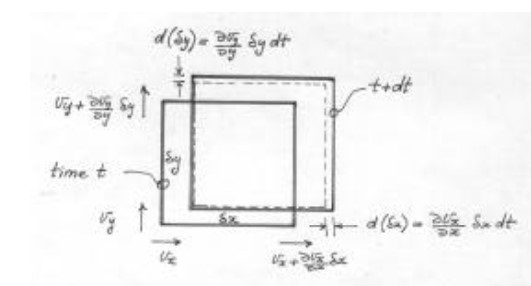
\includegraphics[scale=.9]{Linear Deformation of Fluid Particle.jpg}
\caption{Linear Deformation of Fluid Particle}
\label{fig:Linr_dfrmtn_of_fld_prtcl}
\end{figure}

The linear strain rates can be evaluated in terms of the velocity gradients by referring to Figure \ref{fig:Linr_dfrmtn_of_fld_prtcl}. Between t and t+dt, the linear strain suffered by the fluid particle's side parallel to the $x^{'}$ axis is

$$d\epsilon_{x^{'}} = \frac{\frac{\partial V_{x^{'}}}{\partial x^{'}}\delta x dt}{\delta x} = \frac{\partial V_{x^{'}}}{\partial x^{'}}dt$$

so that 

\begin{equation} \label{e27}
\frac{D\epsilon_{x^{'}}}{Dt} = \frac{\partial V_{x^{'}}}{\partial x^{'}}
\end{equation}

A similar equation is obtained for the linear strain rate in the y' direction. Using these
relations in (\ref{e27}), we now obtain

\begin{equation} \label{e28}
\tau^{'}_{xx} - \tau^{'}_{yy} = 2\mu \bigg(\frac{\partial V_{x^{'}}}{\partial x^{'}} - \frac{\partial V_{y^{'}}}{\partial y^{'}}\bigg)
\end{equation}

Similarly we obtain, by viewing the particle in the ($x^{'}, z^{'}$) plane

\begin{equation} \label{e29}
\tau^{'}_{xx} - \tau^{'}_{zz} = 2\mu \bigg(\frac{\partial V_{x^{'}}}{\partial x^{'}} - \frac{\partial V_{z^{'}}}{\partial z^{'}}\bigg)
\end{equation}

Adding equations (\ref{e28}) and (\ref{e29}) we get

\begin{equation} \label{e30}
\tau_{xx}^{'} = \frac{\tau_{xx}^{'} + \tau_{yy}^{'} + \tau_{zz}^{'}}{3} + 2\mu \frac{\partial V_{x^{'}}}{\partial x^{'}} - \frac{2}{3}\mu \bigg(\frac{\partial V_{x^{'}}}{\partial x^{'}} + \frac{\partial V_{y^{'}}}{\partial y^{'}} + \frac{\partial V_{z^{'}}}{\partial z^{'}}\bigg)
\end{equation}

Since the coordinate system ($x^{'}, y^{'}$) is arbitrary, this relationship must apply in any
coordinate system. We thus have our final result

\begin{equation} \label{e31}
\tau_{xx} = -p_{m} + 2\mu \frac{\partial v_{x}}{\partial x} - \frac{2}{3}\mu \Delta \cdot \overrightarrow{v}
\end{equation}

where the quantity

\begin{equation} \label{e32}
p_{m} = -\frac{\tau_{xx} + \tau_{yy} + \tau_{zz}}{3} = -\frac{\tau_{ij}}{3}
\end{equation}

is the "mechanical" pressure, to be distinguished from the "thermodynamic" pressure
which is discussed below. The mechanical pressure is the negative of the average value of
the three diagonal terms of the stress tensor, and serves as a measure of local normal
compressive stress in viscous flows where that stress is not the same in all directions. The
mechanical pressure is a well defined physical quantity, and is a true scalar since the trace
of a tensor remains invariant under coordinate transformations. Note that although the
definition is phrased in terms of the normal stresses on surfaces pointing in the x, y and z
directions, it can be shown that pm as defined in (\ref{e32}) is in fact equal to the average normal compressive stress on the surface of a sphere centered on the point in question, in the limit as the sphere's radius approaches zero. 

\end{document}

